% file: 3-5-mst/maximal-path-degree-2.tex

\documentclass[tikz]{standalone}

\usetikzlibrary{chains}

\begin{document}
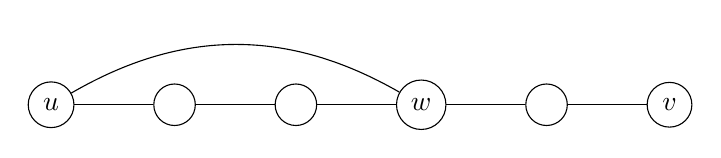
\begin{tikzpicture}[node distance = 1.0cm,
  every node/.style = {draw, circle, minimum size = 15pt},
  every join/.style = {-},
  start chain]
  \foreach \n/\name in {1/u, 2/, 3/, 4/w, 5/, 6/v} {
    \node[on chain, join] {$\name$};
  }

  \draw (chain-1) to [bend left] (chain-4);
\end{tikzpicture}
\end{document}